\section{\texorpdfstring{Phương pháp nghiên cứu}{Method}}
\subsection{\texorpdfstring{Phương pháp đánh giá kết quả nghiên cứu}{Empty}}\label{sec:metrics_eval}
Do đặc thù của bài toán là tạo sinh ảnh mặt người, việc lựa chọn phương pháp để đánh giá chất lượng và độ chân thật của hình ảnh được tạo ra là một thách thức lớn. Dựa trên các tiêu chí về mặt hình ảnh được đưa ra ở phần \ref{target_label}, đoạn còn lại của phần này sẽ đưa ra các độ đo để đo lường chất lượng hình ảnh của mô hình.

Về chất lượng hình ảnh, hầu hết các nghiên cứu trước đây \cite{chen2018}\cite{chen2019}\cite{vougioukas2019}\cite{vougioukas2020} đều sử dụng \textit{Peak Signal-to-Noise Ratio (PSNR)} và \textit{Structural Similarity Index (SSIM)} như các độ đo để đo lường chất lượng hình ảnh được tạo sinh. Tuy nhiên, PSRN lại không phải là một thông số lý tưởng để đo lường khi nó không quan tâm đến các đặc trưng mặt người trong ảnh. Trong khi đó, SSIM lại là một độ đo tốt hơn khi nó có khả năng đo sự tương đồng về mặt nội dung trong ảnh. SSIM có khả năng so sánh các điểm ảnh và các điểm lân cận của chúng trên ảnh được tạo sinh tương ứng với các điểm trên ảnh thật dựa trên ba tính chất - độ tương phản, độ sáng và cấu trúc. Độ nét cũng là một yếu tố quan trọng nói lên chất lượng ảnh. Độ đo Cummulative Probability Blur Detection được sử dụng trong các nghiên cứu \cite{chen2018}\cite{vougioukas2019}\cite{vougioukas2020}
cũng là một độ đo tốt để đánh giá độ nét của ảnh được tạo sinh.

Để đánh giá việc duy trì nhận dạng người trong các hình ảnh được tạo sinh, \textit{Cosin Similarity (CSIM)} là độ đo được sử dụng để đo lường sự sai lệch về nhận dạng trong ảnh được tạo sinh và ảnh thật. Độ đo này đo lường khoảng cách giữa hai vector đặc trưng của hai ảnh thật và tạo sinh, từ đó cho ra một con số cụ thể về sự sai khác giữa hai ảnh.

Sự phù hợp của khẩu hình miệng với từ ngữ được nói ra cũng là một yếu tố quyết định đối với chất lượng ảnh được tạo sinh. Hiện tại, các nghiên cứu đã đưa ra các độ đo khác nhau để đánh giá sự phù hợp này. Trong \cite{vougioukas2019}\cite{vougioukas2020}, tác giả sử dụng độ đo \textit{Word Error Rate (WER)}, trong nghiên cứu này, video mặt người sinh ra được đưa vào LipNet - một mô hình mạng học sâu để đọc từ từ khẩu hình miệng, các từ được đọc ra được so sánh với từ gốc và tính ra tỉ lệ sai. Lele Chen \cite{chen2018} đã đưa ra một độ đo khác để đo lường sự phù hợp khẩu hình miệng là \textit{Landmark Distance (LMD)} nhằm đo lường khoảng cách Euclide giữa các điểm cấu thành khẩu hình miệng trong ảnh thật và ảnh được tạo sinh.

Các độ đo nêu trên là các độ đo đã được kiểm nghiệm tính hiệu quả trong các nghiên cứu gần đây về tạo sinh mặt người dựa vào tiếng nói. Luận văn có thể kế thừa các độ đo này để đánh giá kết quả nghiên cứu, đồng thời có thể dễ dàng so sánh kết quả nghiên cứu của Luận văn với các kết quả nghiên cứu trước đây.

\subsection{\texorpdfstring{Phương pháp thu thập và phân tích số liệu}{Empty}}
Nhằm mục đích dễ dàng cho việc nghiên cứu, đánh giá và so sánh kết quả với các nghiên cứu trước đây, Luận văn sẽ sử dụng các bộ dữ liệu có sẵn, đã được sử dụng trong các nghiên cứu gần đây có cùng chủ đề. Một số tập dữ liệu sau sẽ được sử dụng trong Luận văn:

\textit{GRID}\cite{grid}: Được công bố vào năm 2006, GRID là một tập dữ liệu miễn phí nhằm phục vụ mục đích nghiên cứu. Tập dữ liệu chứa video của 34 người (18 nam, 16 nữ), 1000 video mỗi người, mỗi video có độ dài 3 giây và trong video này, người nói chỉ nói một câu duy nhất.

\textit{CREMA-D}\cite{crema-d}: Được công bố vào năm 2014, CREMA-D là một tập dữ liệu được cung cấp miễn phí cho mục đích nghiên cứu. CREMA-D chứa 7,442 video từ 91 diễn viên, gồm 48 nam và 43 nữ, độ tuổi từ 20 đến 74 từ các chủng tộc người khác nhau. Mỗi diễn viên sẽ nói 12 câu khác nhau, với mỗi câu, họ sẽ thể hiện 6 loại cảm xúc khác nhau khi nói (giận dữ, chán ghét, sợ hãi, vui vẻ, bình thường, và buồn) và 4 cấp độ cảm xúc (thấp, trung bình, cao, và không xác định).

\textit{LRW}\cite{lrw}: Là một bộ dữ liệu lớn được thu thập từ kênh truyền hình BBC, LRW chứa đến hơn 1000 giờ video người đang nói, với bộ từ điển hơn 1000 từ vựng, hơn 1 triệu từ đã được nói bởi hơn 1000 người khác nhau.

\textit{VoxCeleb}\cite{vox}: Tập dữ liệu chứa hơn 100000 từ được nói bởi 1251 người nổi tiếng, những video này được cắt ra từ các video được tải lên YouTube. Tập dữ liệu cũng cân bằng về mặt giới tính với 55\% video là nam. Nhân vật trong video đến từ nhiều chủng tộc khác nhau, ngữ điệu khác nhau, ngành nghề và lứa tuổi cũng khác nhau. Video trong tập dữ liệu cũng được thu thập trong nhiều hoàn cảnh khác nhau (trên thảm đỏ, sân vận động, trong phòng thu,...) và tất cả các video đều được ghi bằng các thiết bị cầm tay.

\begin{figure}[H]
    \centering
    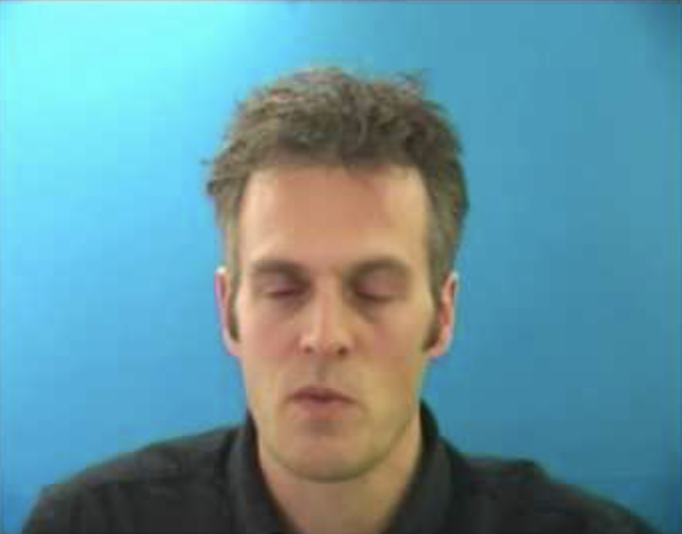
\includegraphics[width=7cm]{./content/images/grid_img.png}
    \caption{Ảnh được cắt từ một video trong tập dữ liệu \textit{GRID}}
\end{figure}

\begin{figure}[H]
    \centering
    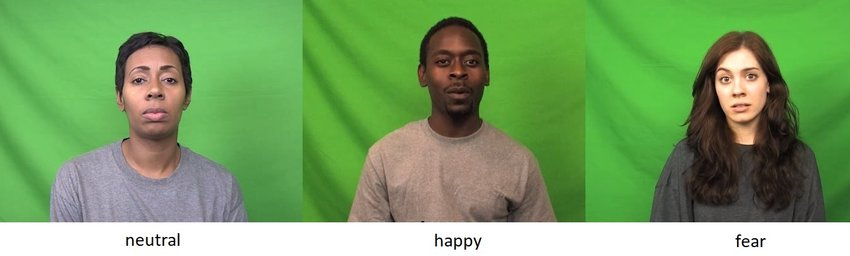
\includegraphics[width=15cm]{./content/images/crema-d_img.jpg}
    \caption{Ảnh được cắt từ các video trong tập dữ liệu \textit{CREMA-D}}
\end{figure}

\begin{figure}[H]
    \centering
    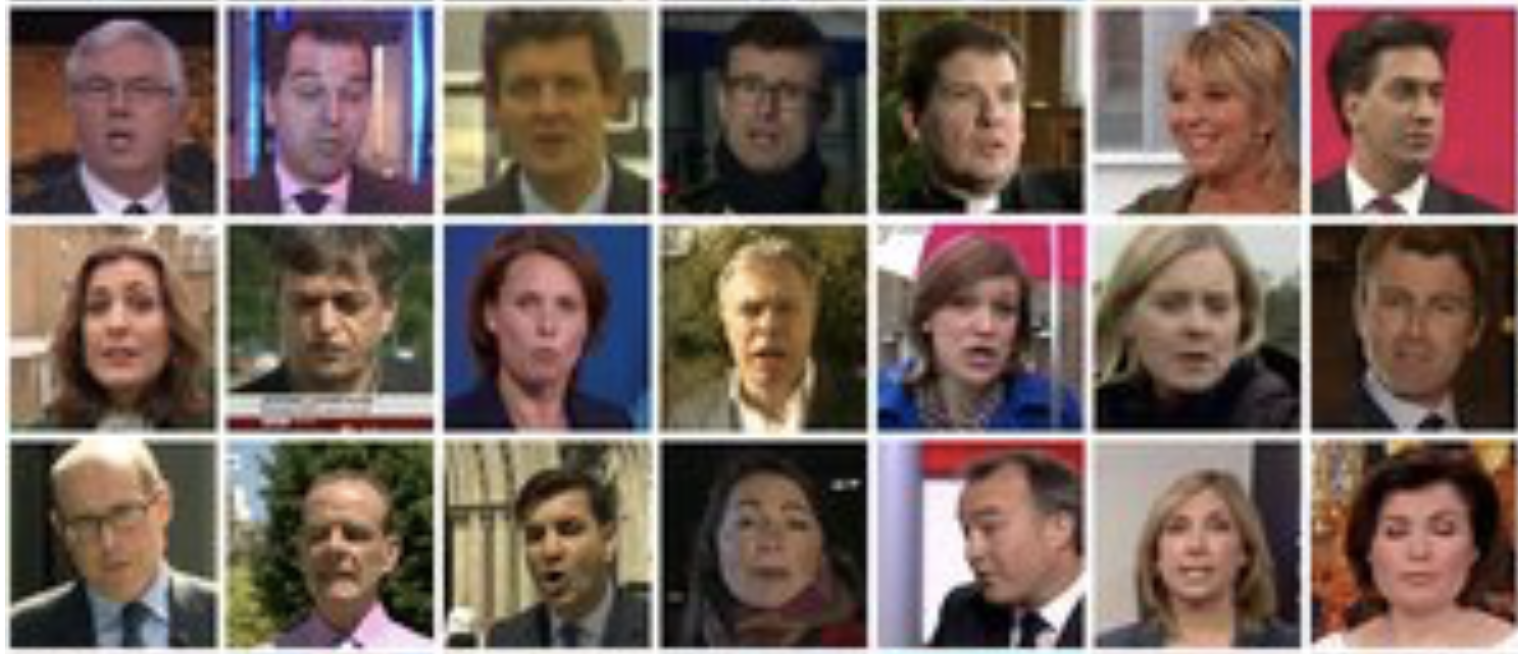
\includegraphics[width=15cm]{./content/images/lrw_img.png}
    \caption{Ảnh được cắt từ các video trong tập dữ liệu \textit{LRW}}
\end{figure}

\begin{figure}[H]
    \centering
    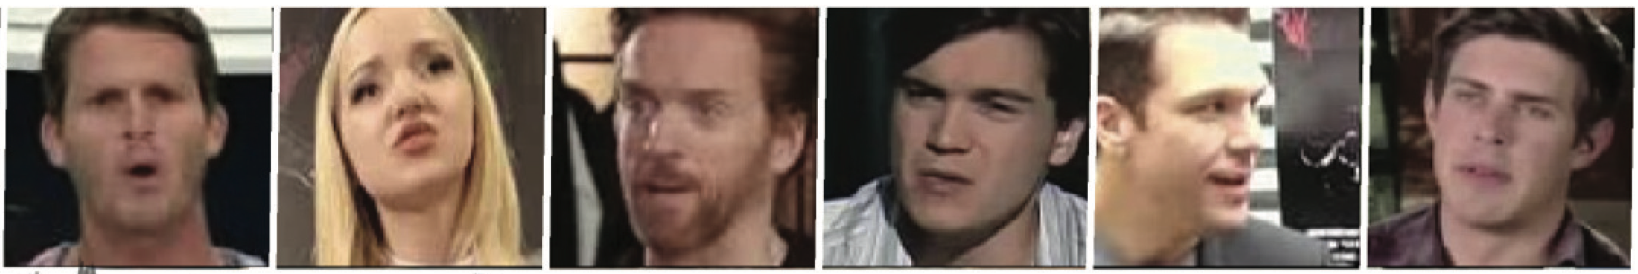
\includegraphics[width=15cm]{./content/images/vox_img.png}
    \caption{Ảnh được cắt từ các video trong tập dữ liệu \textit{VoxCeleb}}
\end{figure}

\subsection{\texorpdfstring{Các thí nghiệm dự kiến sẽ triển khai}{Empty}}

Nhằm mục đích khảo sát, kiểm định và học hỏi, kế thừa các ý tưởng từ các nghiên cứu trước, tác giả sẽ đọc hiểu ý tưởng từ các bài báo từ năm 2018 trở lại đây để nắm rõ lý thuyết và cách vận hành của mô hình được đề ra. Sau đó cài đặt, tiến hành lại các thí nghiệm trên để kiểm chứng và học hỏi thêm kinh nghiệm, đồng thời sẽ cố gắng đề ra những cải tiến cho các mô hình trên nhằm mục đích tăng chất lượng hình ảnh và tính đồng bộ âm thanh cho video được tạo sinh. Từ việc thử nghiệm, cải tiến các mô hình của các nghiên cứu trước, tác giả sẽ thiết kế các mô hình mới và tiến hành thử nghiệm với những cài đặt siêu tham số khác nhau.
